\documentclass[11pt,a4paper]{article}

% ---------- Packages ----------
\usepackage[utf8]{inputenc}
\usepackage[T1]{fontenc}
\usepackage[margin=2.4cm]{geometry}
\usepackage{titlesec}
\usepackage{graphicx}
\usepackage{xcolor}
\usepackage{tikz}
\usetikzlibrary{arrows.meta,positioning,shapes.geometric,fit,backgrounds,decorations.pathreplacing,calc}
\usepackage{pgfgantt}
\usepackage{booktabs}
\usepackage{siunitx}
\usepackage{amsmath,amssymb}
\usepackage{algorithm}
\usepackage{algpseudocode}
\usepackage{enumitem}
\usepackage{hyperref}
\usepackage{caption}
\usepackage{subcaption}
\usepackage{fancyhdr}
\usepackage{longtable}
\usepackage{array}
\usepackage{multirow}
\usepackage{tcolorbox}
\tcbuselibrary{skins,breakable}

% ---------- Colors ----------
\definecolor{primaryblue}{RGB}{31,73,125}
\definecolor{accentteal}{RGB}{0,128,128}
\definecolor{warnred}{RGB}{178,34,34}
\definecolor{softgray}{RGB}{240,240,240}
\definecolor{goodgreen}{RGB}{46,125,50}

\hypersetup{
  colorlinks=true,
  linkcolor=primaryblue,
  citecolor=accentteal,
  urlcolor=accentteal,
  pdftitle={Knowledge-Grounded Zero-Shot Defect Inspection with Confidence-Triggered Revisit Flight for Autonomous UAV Monitoring of Earthen Heritage Architecture},
  pdfauthor={UAS Infrastructure Monitoring Team}
}

\titleformat{\section}{\normalfont\Large\bfseries\color{primaryblue}}{\thesection}{1em}{}
\titleformat{\subsection}{\normalfont\large\bfseries\color{primaryblue}}{\thesubsection}{1em}{}
\titleformat{\subsubsection}{\normalfont\normalsize\bfseries\color{accentteal}}{\thesubsubsection}{1em}{}

\pagestyle{fancy}
\fancyhf{}
\renewcommand{\headrulewidth}{0.4pt}
\fancyhead[L]{\small\itshape Autonomous UAV Inspection of Earthen Heritage Architecture}
\fancyhead[R]{\small\thepage}

\newtcolorbox{keybox}[1]{colback=softgray,colframe=primaryblue,fonttitle=\bfseries,title=#1,breakable}
\newtcolorbox{warnbox}[1]{colback=red!5,colframe=warnred,fonttitle=\bfseries,title=#1,breakable}
\newtcolorbox{riskbox}[1]{colback=orange!5,colframe=orange!70!black,fonttitle=\bfseries,title=#1,breakable}

\newcommand{\code}[1]{\texttt{\small #1}}

\title{
  \vspace{-1.5cm}
  \color{primaryblue}\Huge\bfseries
  Knowledge-Grounded Zero-Shot Defect Inspection\\[0.3em]
  \Large with Confidence-Triggered Revisit Flight\\[0.3em]
  \large for Autonomous UAV Monitoring of Earthen Heritage Architecture
  \vspace{0.3cm}
}
\author{UAS Infrastructure Monitoring Team \\ \small Project Technical Blueprint --- From Zero to Submission}
\date{\small \today}

\begin{document}
\maketitle
\thispagestyle{empty}

\begin{abstract}
\noindent
Autonomous UAV-based inspection of heritage infrastructure typically relies on either (a) geometrically-blind coverage flight paths that ignore what the camera actually sees, or (b) offline defect detectors trained on generic construction materials such as concrete. Both approaches under-serve earthen heritage architecture (mudbrick, pisé, rammed earth), a material class that is structurally distinct from concrete, chronically under-represented in defect-detection literature, and disproportionately at risk given that a significant share of UNESCO-listed heritage sites are built from it. This document specifies a complete, buildable system --- reusing an existing ROS2 + PX4 + Gazebo simulation stack --- that (1) evaluates zero-shot, retrieval-augmented vision-language model (VLM) detection against a domain-specific knowledge base of earthen defect types, (2) compares this against a conventionally-trained YOLOv11 detector on the same material, and (3) introduces a lightweight, detector-agnostic confidence-triggered revisit flight strategy that autonomously re-inspects ambiguous detections at closer range using the platform's existing A* planner. The contribution is explicitly framed as a \emph{comparative empirical study} across six detection-and-strategy combinations rather than a claim of algorithmic novelty, since the underlying techniques (RAG-grounded VLM inspection, active 3D reconstruction, semantic path planning) are each independently established in recent literature. This document specifies the full system architecture, the mathematical formulation of every subsystem, the dataset and knowledge-base construction process, a from-zero setup and installation guide, a day-by-day execution plan for a 25--30 day sprint, and the evaluation protocol required to produce a defensible conference submission.
\end{abstract}

\vspace{0.5cm}
\begin{keybox}{Document Scope}
This is a \emph{project blueprint}, not a finished paper. Every section is written so that a four-person team with no prior experience in retrieval-augmented VLMs can go from an empty repository to a submittable manuscript. Figures marked \emph{(illustrative)} show the intended shape of a result; they must be replaced with real experimental output before submission.
\end{keybox}

\newpage
\tableofcontents
\newpage

% =====================================================================
\section{Motivation and Problem Statement}
% =====================================================================

\subsection{Why the original scope is not enough}

The team's original prototype scope (Figure~\ref{fig:original-pipeline}) executes a fixed geometric lawnmower scan and runs a single, offline-trained YOLOv11 model on the recorded footage after the flight has ended. This is a sound engineering integration exercise, but it is not a research contribution: the flight path never reacts to what the camera sees, and the detector has no relationship to the specific material being inspected.

\begin{figure}[h!]
\centering
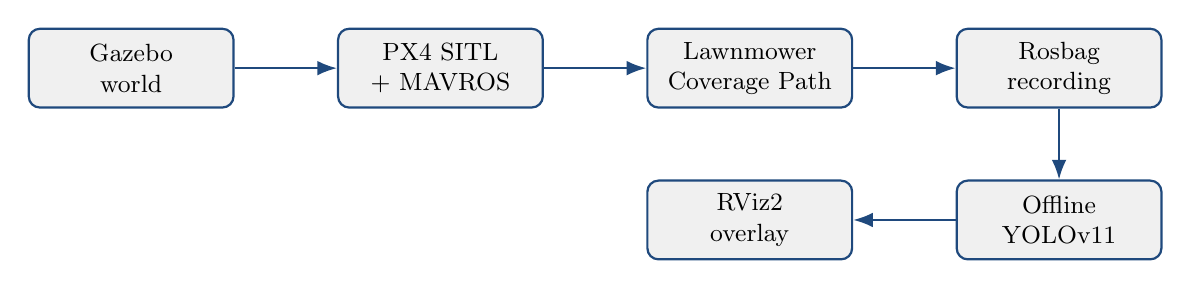
\begin{tikzpicture}[
  node distance=0.9cm and 1.3cm,
  block/.style={rectangle, draw=primaryblue, thick, rounded corners, fill=softgray, minimum width=2.6cm, minimum height=1cm, align=center, font=\small},
  arrow/.style={-{Latex[length=2.5mm]}, thick, primaryblue}
]
\node[block] (gz) {Gazebo\\ world};
\node[block, right=of gz] (px4) {PX4 SITL\\ + MAVROS};
\node[block, right=of px4] (cpp) {Lawnmower\\ Coverage Path};
\node[block, right=of cpp] (bag) {Rosbag\\ recording};
\node[block, below=of bag] (yolo) {Offline\\ YOLOv11};
\node[block, left=of yolo] (rviz) {RViz2\\ overlay};

\draw[arrow] (gz) -- (px4);
\draw[arrow] (px4) -- (cpp);
\draw[arrow] (cpp) -- (bag);
\draw[arrow] (bag) -- (yolo);
\draw[arrow] (yolo) -- (rviz);
\end{tikzpicture}
\caption{Original Phase 1 scope: a closed loop that never reacts to what it sees. Detection happens strictly after the flight is over.}
\label{fig:original-pipeline}
\end{figure}

\subsection{The two real gaps}

A literature review (Section~\ref{sec:relatedwork}) rules out several tempting ``novel'' pivots as already saturated: semantic-driven active path planning, live A* preemption, and active 3D Gaussian Splatting reconstruction are all established research directions with multiple 2020--2025 publications. Two gaps, however, remain genuinely open:

\begin{enumerate}
    \item \textbf{Material gap.} Automated crack and defect detection for earthen/rammed-earth/mudbrick heritage architecture is a thin literature, and every existing study operates on static photographs. None integrate with an autonomous flight platform.
    \item \textbf{Method-transfer gap.} Retrieval-augmented, knowledge-grounded zero-shot VLM inspection is a real and very recent technique (first demonstrated for wind turbine blades in October 2025), but has never been applied to earthen heritage, nor embedded in a closed UAV flight loop.
\end{enumerate}

\begin{keybox}{Honest Novelty Statement}
This project does not claim to invent a new detection algorithm, a new path-planning algorithm, or a new 3D reconstruction technique. Its contribution is an \emph{empirical comparative study}: which detection paradigm (raw zero-shot VLM, RAG-grounded VLM, trained YOLOv11) and which inspection strategy (single-pass vs. confidence-triggered revisit) performs best for autonomous earthen-heritage inspection --- a question nobody has answered, because nobody has run this comparison on this material class inside a flight loop.
\end{keybox}

% =====================================================================
\section{Related Work}
\label{sec:relatedwork}
% =====================================================================

Table~\ref{tab:relatedwork} summarizes the literature this project builds on and is positioned against. Every claim of ``the gap'' made in Section 1 is directly traceable to this table --- this is also the material for the paper's own Related Work section.

\begin{table}[h!]
\centering
\small
\begin{tabular}{p{2.6cm} p{6.3cm} p{4.6cm}}
\toprule
\textbf{Area} & \textbf{What exists} & \textbf{What is missing} \\
\midrule
Semantic active path planning & Bartolomei et al. (IROS 2021) close the loop between semantic detection and UAV trajectory. & Already established; not usable as the paper's central claim. \\
\addlinespace
Real-time UAV crack inspection & A 2023 \emph{Sensors} paper runs live crack detection with 2D--3D projection on a Jetson-class UAV. & Same architecture as above; concrete/generic materials only. \\
\addlinespace
Active 3D Gaussian Splatting reconstruction & ActiveGS (RA-L 2025), GS-Planner (IROS 2024), DroneSplat (CVPR 2025) actively select UAV viewpoints to optimize live 3DGS reconstruction. & A mature, sophisticated subfield --- too saturated and too research-heavy to match in a short sprint. \\
\addlinespace
Zero-shot VLM defect detection & RareCLIP (ICCV 2025), ID-RAG, AnomalyGPT, FabGPT and others detect industrial anomalies zero-shot. & Applied to manufacturing/industrial surfaces, not heritage or earthen materials. \\
\addlinespace
Knowledge-grounded RAG+VLM inspection & A wind-turbine blade inspection paper (arXiv 2510.22868, Oct.\ 2025) grounds a VLM with a retrieved multimodal knowledge base for zero-shot defect classification. & The closest prior work; never applied outside wind-turbine composites, never flown on a UAV. \\
\addlinespace
Earthen heritage crack detection & SVM-based detection on rammed earth (2020); FPN-VGG16 pixel-level segmentation on earthen heritage (2022); YOLO material comparison across historic building materials (2024, earthen scoring lowest of all tested materials at 81.6\% mAP). & Static photographs only. No flight platform. No zero-shot / RAG methods applied to this material. \\
\bottomrule
\end{tabular}
\caption{Positioning of this project against existing literature. Each row is independently citable.}
\label{tab:relatedwork}
\end{table}

% =====================================================================
\section{System Architecture}
% =====================================================================

\subsection{Overview}

Figure~\ref{fig:architecture} shows the full system. The shaded region marks the components that are new; everything outside it is reused, unmodified, from the existing ROS2/PX4/Gazebo prototype.

\begin{figure}[h!]
\centering
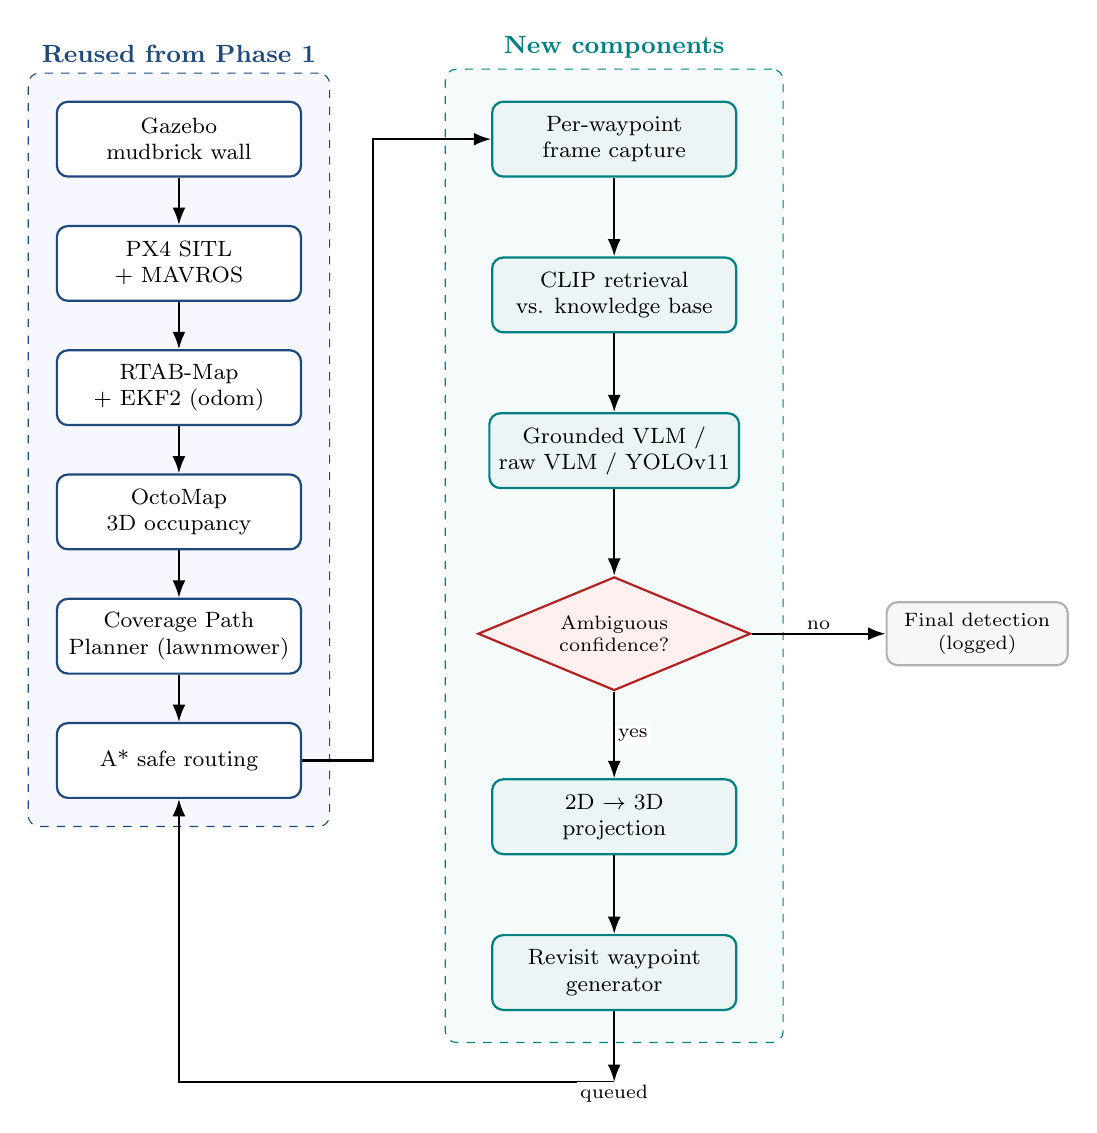
\begin{tikzpicture}[
  node distance=0.6cm and 2.4cm,
  block/.style={rectangle, draw=primaryblue, thick, rounded corners, fill=white, minimum width=3.1cm, minimum height=0.95cm, align=center, font=\footnotesize},
  newblock/.style={rectangle, draw=accentteal, thick, rounded corners, fill=teal!8, minimum width=3.1cm, minimum height=0.95cm, align=center, font=\footnotesize},
  decision/.style={diamond, draw=warnred, thick, fill=red!6, aspect=2.4, minimum width=3.4cm, text width=1.9cm, align=center, font=\scriptsize, inner sep=2pt},
  arrow/.style={-{Latex[length=2.2mm]}, thick},
  lbl/.style={font=\scriptsize, fill=white, inner sep=1pt},
  every node/.style={font=\footnotesize}
]

\node[block] (gz) {Gazebo\\ mudbrick wall};
\node[block, below=of gz] (px4) {PX4 SITL\\ + MAVROS};
\node[block, below=of px4] (odom) {RTAB-Map\\ + EKF2 (odom)};
\node[block, below=of odom] (octo) {OctoMap\\ 3D occupancy};
\node[block, below=of octo] (cpp) {Coverage Path\\ Planner (lawnmower)};
\node[block, below=of cpp] (astar) {A* safe routing};

\node[newblock, right=of gz] (capture) {Per-waypoint\\ frame capture};
\node[newblock, below=1.0cm of capture] (clip) {CLIP retrieval\\ vs. knowledge base};
\node[newblock, below=1.0cm of clip] (vlm) {Grounded VLM /\\ raw VLM / YOLOv11};
\node[decision, below=1.1cm of vlm] (conf) {Ambiguous confidence?};
\node[newblock, below=1.1cm of conf] (proj) {2D $\rightarrow$ 3D\\ projection};
\node[newblock, below=1.0cm of proj] (revisit) {Revisit waypoint\\ generator};
\node[rectangle, draw=gray!60, thick, rounded corners, fill=gray!6, minimum width=2.3cm, minimum height=0.8cm, align=center, font=\scriptsize, right=1.7cm of conf] (final) {Final detection\\ (logged)};

\draw[arrow] (gz) -- (px4);
\draw[arrow] (px4) -- (odom);
\draw[arrow] (odom) -- (octo);
\draw[arrow] (octo) -- (cpp);
\draw[arrow] (cpp) -- (astar);

\draw[arrow] (astar.east) -- ++(0.9,0) |- (capture.west);
\draw[arrow] (capture) -- (clip);
\draw[arrow] (clip) -- (vlm);
\draw[arrow] (vlm) -- (conf);
\draw[arrow] (conf.south) -- (proj.north) node[lbl, midway, right]{yes};
\draw[arrow] (conf.east) -- (final.west) node[lbl, midway, above]{no};

\draw[arrow] (proj) -- (revisit);
\coordinate (qbend) at ($(revisit.south)+(0,-0.9)$);
\draw[arrow] (revisit.south) -- (qbend);
\draw[arrow] (qbend) -| (astar.south);
\node[lbl, below] at (qbend) {queued};

\begin{scope}[on background layer]
\node[fit=(capture)(clip)(vlm)(conf)(proj)(revisit), inner sep=0.4cm, fill=teal!4, draw=accentteal, dashed, rounded corners, label={[accentteal, font=\bfseries\small]above:New components}] {};
\node[fit=(gz)(px4)(odom)(octo)(cpp)(astar), inner sep=0.35cm, fill=blue!3, draw=primaryblue, dashed, rounded corners, label={[primaryblue, font=\bfseries\small]above:Reused from Phase 1}] {};
\end{scope}

\end{tikzpicture}
\caption{Full system architecture. The revisit waypoint generator is the only component that feeds back into the existing A* planner --- no new planning algorithm is introduced. A confirmed (``no'') detection is simply logged as final; only ambiguous (``yes'') detections trigger a queued revisit route.}
\label{fig:architecture}
\end{figure}

\subsection{Design principle: decoupled logging and inference rate}
\label{sec:decoupled}

A critical, easy-to-miss design decision: the rosbag records at full sensor rate (commonly 30\,fps) because odometry and mapping need temporal density. Defect detection does not need this density --- it needs one look per patch of wall. Running a VLM on every recorded frame is therefore both unnecessary and prohibitively slow (see cost model below). Instead, one frame is captured per coverage waypoint, decoupling the two rates entirely.

\begin{keybox}{Worked Cost Comparison}
\textbf{Naive (wrong) design:} 30\,fps $\times$ 10 minutes = 18{,}000 frames. At $\sim$0.5\,s/frame for a VLM forward pass, that is $\sim$2.5 hours of processing for a 10-minute flight.\\[4pt]
\textbf{Waypoint-decoupled design:} A coverage plan with $N=\lceil H/d_{overlap}\rceil$ strips over a realistic facade yields on the order of 100--150 total waypoints. At 0.5\,s/frame, total inference cost is $\sim$75 seconds, run once, after the flight.
\end{keybox}

% =====================================================================
\section{Datasets and Knowledge Base}
% =====================================================================

\begin{table}[h!]
\centering
\small
\begin{tabular}{p{3.4cm}p{5.2cm}p{5.2cm}}
\toprule
\textbf{Asset} & \textbf{Purpose} & \textbf{Source / Construction} \\
\midrule
SDNET2018 & Baseline concrete crack imagery; used both for YOLOv11 supervised baseline and as source crops for the RAG knowledge base & Existing, already downloaded \\
MBDD2025 & Aerial defect imagery, closer to UAV viewing angle & Existing, already downloaded \\
Gazebo mudbrick wall (extended) & Simulation testbed with procedurally placed crack morphologies (hairline/network, spalling, erosion) & Extend existing world; texture patterns informed by published earthen-heritage crack figures \\
RAG knowledge base & 20--40 curated entries: short paraphrased textual description of each defect class + 3--5 reference image crops per class & Manual curation from literature descriptions and existing dataset crops --- no training required \\
Hand-labeled evaluation set & 30--50 frames from Gazebo flights, manually annotated with known crack locations & Built in-house, since crack placement in simulation is already known \\
\bottomrule
\end{tabular}
\caption{Data assets required. Note that the zero-shot VLM conditions require \emph{no} labeled training set --- only the YOLOv11 baseline condition and the evaluation set need labels.}
\label{tab:datasets}
\end{table}

\begin{figure}[h!]
\centering
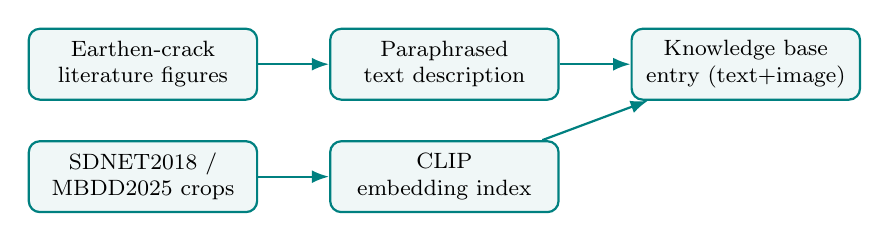
\begin{tikzpicture}[
  node distance=0.5cm and 0.9cm,
  block/.style={rectangle, draw=accentteal, thick, rounded corners, fill=teal!6, minimum width=2.9cm, minimum height=0.9cm, align=center, font=\footnotesize},
  arrow/.style={-{Latex[length=2.2mm]}, thick, accentteal}
]
\node[block] (lit) {Earthen-crack\\ literature figures};
\node[block, right=of lit] (desc) {Paraphrased\\ text description};
\node[block, below=of lit] (crops) {SDNET2018 /\\ MBDD2025 crops};
\node[block, right=of crops] (embed) {CLIP\\ embedding index};
\node[block, right=of desc] (kb) {Knowledge base\\ entry (text+image)};

\draw[arrow] (lit) -- (desc);
\draw[arrow] (crops) -- (embed);
\draw[arrow] (desc) -- (kb);
\draw[arrow] (embed) -- (kb);
\end{tikzpicture}
\caption{Knowledge-base construction pipeline. This is a curation task (1--2 days), not a training run.}
\label{fig:kb}
\end{figure}

% =====================================================================
\section{Algorithms, End to End}
% =====================================================================

\subsection{A. Odometry (reused, unmodified)}
The Extended Kalman Filter fuses visual pose estimate $z_k$ with IMU-propagated state:
\begin{equation}
x_{k|k} = x_{k|k-1} + K_k\left(z_k - H x_{k|k-1}\right), \qquad
K_k = P_{k|k-1}H^\top\left(HP_{k|k-1}H^\top + R\right)^{-1}
\end{equation}

\subsection{B. Coverage path planning (reused, unmodified)}
For a facade of height $H$ and vertical camera footprint $h_{FOV}$ at standoff $D$, with overlap ratio $\rho = 0.3$:
\begin{equation}
N = \left\lceil \frac{H}{d_{overlap}} \right\rceil, \qquad d_{overlap} = h_{FOV}\times(1-\rho)
\end{equation}

\begin{figure}[h!]
\centering
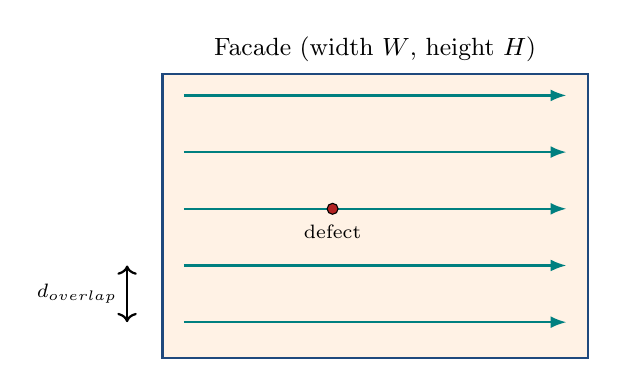
\begin{tikzpicture}[scale=0.9]
\draw[fill=orange!10, draw=primaryblue, thick] (0,0) rectangle (6,4);
\node[font=\small] at (3,4.35) {Facade (width $W$, height $H$)};
\foreach \y in {0.5,1.3,2.1,2.9,3.7} {
  \draw[-{Latex[length=2mm]}, thick, accentteal] (0.3,\y) -- (5.7,\y);
}
\draw[<->, thick] (-0.5,0.5) -- (-0.5,1.3) node[midway, left, font=\scriptsize]{$d_{overlap}$};
\draw[fill=warnred] (2.4,2.1) circle (2.2pt);
\node[font=\scriptsize, below=1pt] at (2.4,2.05) {defect};
\end{tikzpicture}
\caption{Lawnmower coverage pattern (reused, unmodified). Each horizontal strip becomes a sequence of waypoints; one frame is captured per waypoint (Section~\ref{sec:decoupled}).}
\label{fig:lawnmower}
\end{figure}

\subsection{C. A* safe routing (reused, unmodified)}
Standard grid-search shortest-path routing over OctoMap occupancy voxels. Used identically for (i) the primary lawnmower pass and (ii) any revisit-leg waypoints --- no modification to this node is required.

\subsection{D. Retrieval-augmented grounding (new)}
Given a live frame $I$, embed it with a CLIP image encoder $\phi(\cdot)$ and retrieve the top-$k$ knowledge-base entries by cosine similarity against pre-computed knowledge-base embeddings $\{\phi(e_i)\}$:
\begin{equation}
\text{retrieve}(I) = \operatorname*{arg\,top\text{-}k}_{i} \; \frac{\phi(I)\cdot\phi(e_i)}{\lVert\phi(I)\rVert\,\lVert\phi(e_i)\rVert}
\end{equation}
The retrieved text descriptions and reference crops are concatenated into a grounded prompt for the VLM.

\subsection{E. Detection (three interchangeable conditions)}
\begin{itemize}[leftmargin=1.3cm]
    \item[\textbf{Condition A}] Raw zero-shot VLM: prompt with generic defect-class names, no retrieval.
    \item[\textbf{Condition B}] RAG-grounded VLM: prompt constructed from Section D's retrieval.
    \item[\textbf{Condition C}] Trained YOLOv11: conventionally supervised on SDNET2018 + MBDD2025 (+earthen augmentation).
\end{itemize}
All three expose a common interface: bounding box, defect class, confidence $C \in [0,1]$.

\subsection{F. 2D $\rightarrow$ 3D projection (reused pinhole math, unmodified)}
\begin{equation}
Z = D(u,v), \qquad
X = \frac{(u-c_x)Z}{f_x}, \qquad
Y = \frac{(v-c_y)Z}{f_y}
\end{equation}

\subsection{G. Confidence-triggered revisit (new, detector-agnostic)}
\begin{equation}
D_{revisit} = \max\left(D_{min},\; D_{base} - k(1-C)\right)
\end{equation}
Triggered only when $C \in [\tau_l, \tau_h]$ (ambiguous band, e.g. $[0.4, 0.7]$). Revisit waypoints are computed \emph{after} the primary pass completes and routed through the existing A* planner --- there is no live interruption of the in-progress flight.

\begin{algorithm}[h!]
\caption{Post-flight revisit pass (detector-agnostic)}
\begin{algorithmic}[1]
\State $D \gets$ \Call{RunDetectorOnWaypointFrames}{primary\_pass\_frames}
\State $Q \gets \emptyset$ \Comment{revisit queue}
\For{each detection $d \in D$}
    \If{$\tau_l \le d.\text{confidence} \le \tau_h$}
        \State $p_{3D} \gets$ \Call{ProjectTo3D}{$d.\text{bbox}$, depth\_frame}
        \State $D_{revisit} \gets \max(D_{min}, D_{base} - k(1 - d.\text{confidence}))$
        \State $Q \gets Q \cup \{(p_{3D}, D_{revisit})\}$
    \EndIf
\EndFor
\State $\text{route} \gets$ \Call{AStar}{OctoMap, $Q$} \Comment{reused planner, unmodified}
\State \Call{FlyRoute}{route}
\State $D' \gets$ \Call{RunDetectorOnWaypointFrames}{revisit\_frames}
\State \Return $D \cup D'$ \Comment{final detections, with confidence deltas logged}
\end{algorithmic}
\end{algorithm}

% =====================================================================
\section{The Comparative Study Design}
% =====================================================================

The central empirical contribution is a full factorial comparison of three detection paradigms against two inspection strategies (Figure~\ref{fig:matrix}). This directly answers the anticipated review/jury critique --- ``anyone can call a VLM on an image'' --- by making the comparison itself the result, rather than the pipeline being the result.

\begin{figure}[h!]
\centering
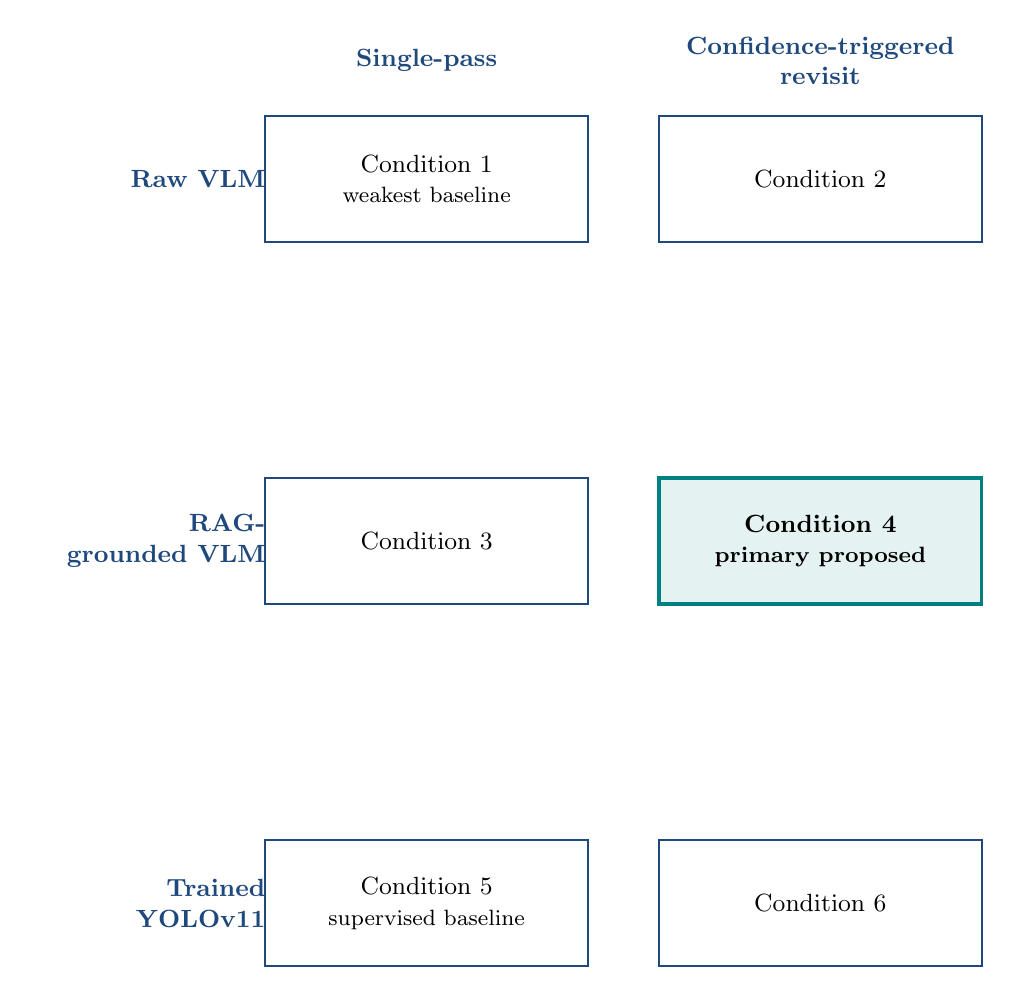
\begin{tikzpicture}[
  cell/.style={rectangle, draw=primaryblue, thick, minimum width=4.1cm, minimum height=1.6cm, align=center, font=\small},
  hicell/.style={rectangle, draw=accentteal, very thick, fill=teal!10, minimum width=4.1cm, minimum height=1.6cm, align=center, font=\small\bfseries},
  collbl/.style={font=\small\bfseries, primaryblue, align=center},
  rowlbl/.style={font=\small\bfseries, primaryblue, align=right, text width=2.9cm}
]
\coordinate (r1) at (0,4.6);
\coordinate (r2) at (0,0);
\coordinate (r3) at (0,-4.6);
\coordinate (c1) at (0,0);
\coordinate (c2) at (5.0,0);

\node[collbl] at ($(c1)+(0,6.1)$) {Single-pass};
\node[collbl] at ($(c2)+(0,6.1)$) {Confidence-triggered\\ revisit};

\node[rowlbl] at (-3.5,4.6) {Raw VLM};
\node[rowlbl] at (-3.5,0) {RAG-grounded VLM};
\node[rowlbl] at (-3.5,-4.6) {Trained YOLOv11};

\node[cell] at (0,4.6)  {Condition 1\\ \footnotesize weakest baseline};
\node[cell] at (5.0,4.6) {Condition 2};
\node[cell] at (0,0)    {Condition 3};
\node[hicell] at (5.0,0) {Condition 4\\ \footnotesize primary proposed};
\node[cell] at (0,-4.6) {Condition 5\\ \footnotesize supervised baseline};
\node[cell] at (5.0,-4.6) {Condition 6};
\end{tikzpicture}
\caption{Six-condition comparative matrix. The revisit strategy is detector-agnostic and reuses the same code path across all three detectors --- this is itself a methodological point worth stating explicitly in the paper.}
\label{fig:matrix}
\end{figure}

\subsection{Metrics collected per condition}
\begin{itemize}
    \item Precision / recall against the hand-labeled evaluation set
    \item Confidence gain on revisit vs.\ first pass (revisit conditions only)
    \item Effective resolution (pixels-per-metric, PPM) on flagged defects
    \item Inference cost per waypoint (ms) --- turns the earlier VLM-speed concern into a reported accuracy/latency trade-off rather than an unresolved risk
    \item Total flight-time overhead of revisit vs.\ single-pass
\end{itemize}

\begin{figure}[h!]
\centering
\begin{tikzpicture}
\begin{scope}
\draw[->, thick] (0,0) -- (8,0) node[right, font=\small]{Recall};
\draw[->, thick] (0,0) -- (0,5) node[above, font=\small]{Inference cost (ms/waypoint)};
\node[draw=primaryblue, fill=blue!10, circle, minimum size=6pt, inner sep=0pt] at (1.5,1.0) {};
\node[font=\scriptsize, below] at (1.5,0.9) {C1: raw VLM};
\node[draw=accentteal, fill=teal!15, circle, minimum size=6pt, inner sep=0pt] at (4.2,2.6) {};
\node[font=\scriptsize, above] at (4.2,2.7) {C4: RAG+revisit};
\node[draw=orange!80!black, fill=orange!15, circle, minimum size=6pt, inner sep=0pt] at (6.0,1.4) {};
\node[font=\scriptsize, below] at (6.0,1.3) {C6: YOLO+revisit};
\node[font=\scriptsize, gray, rotate=25] at (5,4) {\emph{(illustrative --- replace with real data)}};
\end{scope}
\end{tikzpicture}
\caption{Illustrative accuracy/latency trade-off plot --- the intended shape of the paper's headline figure. Populate with real measurements from Section~\ref{sec:eval}.}
\label{fig:tradeoff}
\end{figure}

% =====================================================================
\section{Setup Guide: From Zero to Running System}
% =====================================================================

This section assumes an empty machine. It reuses the team's existing Docker-based simulation stack (\code{setup.md}) and layers the new components on top.

\subsection{Step 1 --- Host prerequisites (Linux / Fedora reference)}
\begin{verbatim}
sudo systemctl enable --now docker
sudo usermod -aG docker "$USER"
newgrp docker
sudo dnf install xorg-x11-server-utils
xhost +local:
\end{verbatim}
Windows teammates use the \code{sim-headless} or \code{sim-novnc} Docker Compose profiles instead of host X11 (see \code{setup.md}, Windows section).

\subsection{Step 2 --- Build and start the simulation stack}
\begin{verbatim}
docker compose build sim_stack
docker compose --profile sim up -d
docker exec -it uas_sim bash -lc "/home/uas/scripts/bootstrap_px4.sh"
\end{verbatim}

\subsection{Step 3 --- Launch PX4 + Gazebo + MAVROS + camera bridge}
\begin{verbatim}
PX4_GZ_WORLD=obstacle_maze PX4_GZ_MODEL_TARGET=gz_x500_mono_cam \
  ./scripts/launch_obstacle_stack.sh
\end{verbatim}
This opens the four-window tmux session: PX4+Gazebo, MAVROS, camera bridge, flight script. Verify camera topics:
\begin{verbatim}
ros2 topic list | grep -Ei "camera|image|depth|points"
\end{verbatim}

\subsection{Step 4 --- New component: RAG knowledge base}
\begin{enumerate}
    \item Curate 20--40 entries (Section 4, Figure~\ref{fig:kb}) as a simple JSON/YAML file: \code{\{class, text\_description, image\_crop\_paths[]\}}.
    \item Compute and cache CLIP embeddings for every entry offline --- this only needs to run once.
    \item Store the resulting embedding index alongside the knowledge base file; load both at node startup.
\end{enumerate}

\subsection{Step 5 --- New component: detection node}
Implement one ROS2 node exposing a common detection interface, with three interchangeable backends selected by a launch argument (\code{raw\_vlm}, \code{rag\_vlm}, \code{yolo}). The node subscribes to the camera topic but only processes a frame when triggered by waypoint arrival (Section~\ref{sec:decoupled}), not on every published frame.

\subsection{Step 6 --- New component: revisit waypoint generator}
A small ROS2 node that: (i) consumes detection output plus depth for 3D projection, (ii) filters by the ambiguous confidence band, (iii) computes $D_{revisit}$, (iv) publishes a new waypoint list to the existing A* planner. No modification to the A* or OctoMap nodes themselves.

\subsection{Step 7 --- Data recording (reused)}
\begin{verbatim}
export MAVROS_NS=/uas1
python3 /home/uas/scripts/fly_pattern.py
\end{verbatim}
Bags are written to \code{shared/rosbags/}; analysis via \code{analyze\_rosbags.py} is unchanged.

\subsection{Step 8 --- Running all six conditions}
Re-run the same flight (or replay the same rosbag frames) with each of the six \code{(detector, strategy)} launch configurations. Score each against the shared hand-labeled evaluation set.

\begin{warnbox}{Common Pitfalls (from the team's own troubleshooting log)}
\begin{itemize}[leftmargin=1.2cm]
    \item \code{PX4 server already running for instance 0} --- kill stale processes or \code{docker restart uas\_sim} before relaunching.
    \item MAVROS must start \emph{after} PX4 is fully up, and \emph{before} the flight/detection script, or topics under \code{/uas1/...} will not exist yet.
    \item Do not set \code{COM\_ARM\_EKF\_*} to \code{0} --- PX4 treats these as maximum innovation thresholds; \code{0} makes arming stricter, not looser.
    \item Camera/depth topics only appear once a camera-equipped model (\code{gz\_x500\_mono\_cam} or \code{gz\_x500\_depth}) is launched --- the base \code{gz\_x500} has no camera.
\end{itemize}
\end{warnbox}

% =====================================================================
\section{Execution Plan (25--30 Days)}
% =====================================================================

\begin{figure}[h!]
\centering
\resizebox{\textwidth}{!}{%
\begin{ganttchart}[
    vgrid, hgrid,
    x unit=0.42cm,
    y unit chart=0.7cm,
    bar/.append style={fill=accentteal},
    bar height=0.55,
    group/.append style={fill=primaryblue},
    milestone/.append style={fill=warnred},
    title height=1,
    bar label font=\scriptsize,
    group label font=\bfseries\scriptsize,
    title label font=\bfseries\scriptsize
]{1}{30}
\gantttitle{25--30 Day Sprint}{30} \\
\gantttitlelist{1,...,30}{1} \\
\ganttgroup{Sim/Nav track}{1}{18} \\
\ganttbar{Re-verify base stack}{1}{4} \\
\ganttbar{Extend wall crack morphologies}{5}{9} \\
\ganttbar{Revisit waypoint generator}{10}{18} \\
\ganttgroup{Data track}{1}{22} \\
\ganttbar{Curate RAG knowledge base}{1}{9} \\
\ganttbar{Earthen-augment YOLO dataset}{5}{9} \\
\ganttbar{Build hand-labeled eval set}{19}{22} \\
\ganttgroup{AI track}{1}{24} \\
\ganttbar{Raw VLM stood up}{1}{4} \\
\ganttbar{RAG grounding added}{5}{9} \\
\ganttbar{YOLOv11 training (parallel)}{5}{14} \\
\ganttbar{Common detector interface}{10}{18} \\
\ganttbar{Integration test, 6 conditions}{19}{24} \\
\ganttgroup{Evaluation \& writing}{19}{30} \\
\ganttbar{Run all 6 conditions in Gazebo}{19}{24} \\
\ganttbar{Score against eval set}{22}{25} \\
\ganttbar{Paper writing \& submission}{25}{30} \\
\ganttmilestone{Submission deadline}{30}
\end{ganttchart}
}
\caption{Day-by-day execution plan across the original four-person track split (Simulation, Navigation, Data, AI).}
\label{fig:gantt}
\end{figure}

\begin{table}[h!]
\centering
\small
\begin{tabular}{p{1.4cm}p{2.4cm}p{2.4cm}p{2.4cm}p{2.4cm}}
\toprule
\textbf{Days} & \textbf{Sim} & \textbf{Nav} & \textbf{Data} & \textbf{AI} \\
\midrule
1--4 & Re-verify base stack & same & Curate RAG knowledge base & Stand up raw VLM (Condition 1) \\
5--9 & Add crack morphologies & --- & Earthen-augment YOLO dataset (parallel) & Add RAG grounding; start YOLOv11 training \\
10--14 & --- & Build revisit generator & Finish augmentation & Finish YOLOv11; unify detector interface \\
15--18 & --- & Wire revisit to all 3 detectors & Build eval set & Integration test individually \\
19--24 & Run all 6 conditions & Validate trajectories & Score conditions & Debug/rerun \\
25--30 & \multicolumn{4}{l}{All: writing --- results table is the spine of the paper} \\
\bottomrule
\end{tabular}
\caption{Same plan in tabular form, cross-referenced to Figure~\ref{fig:gantt}.}
\end{table}

\begin{riskbox}{If Time Runs Short --- Cut Order}
Drop, in this order, if the schedule slips: (1) Condition 2 (raw VLM + revisit --- least informative), (2) reduce evaluation set size rather than skipping an entire condition, (3) as a last resort, drop Condition 5/6 revisit legs but \emph{keep} the single-pass YOLO baseline, since it is the cheapest to run and anchors the comparison. Do not cut the RAG-grounded conditions (3, 4) or the raw-VLM baseline (1) --- these are the actual paper.
\end{riskbox}

% =====================================================================
\section{Evaluation Protocol}
\label{sec:eval}
% =====================================================================

\begin{table}[h!]
\centering
\small
\begin{tabular}{lcccccc}
\toprule
\textbf{Condition} & \textbf{Detector} & \textbf{Strategy} & \textbf{Precision} & \textbf{Recall} & \textbf{ms/frame} & \textbf{Flight $\Delta$} \\
\midrule
1 & Raw VLM & Single-pass & -- & -- & -- & -- \\
2 & Raw VLM & Revisit & -- & -- & -- & -- \\
3 & RAG VLM & Single-pass & -- & -- & -- & -- \\
4 & RAG VLM & Revisit & -- & -- & -- & -- \\
5 & YOLOv11 & Single-pass & -- & -- & -- & -- \\
6 & YOLOv11 & Revisit & -- & -- & -- & -- \\
\bottomrule
\end{tabular}
\caption{Results table template --- the direct deliverable of Section~\ref{sec:eval}. Populate every cell with measured values before submission; do not publish with placeholders.}
\label{tab:resultstemplate}
\end{table}

\subsection{The jury question, answered in advance}
\begin{keybox}{``Isn't this just asking a VLM to detect cracks --- anyone could do that?''}
Correct that calling a pretrained VLM on an image is not, by itself, a contribution. The contribution is threefold: (1) measuring \emph{whether} retrieval grounding actually helps on this specific under-studied material class (Condition~1 vs.~3), (2) measuring whether a lightweight, detector-agnostic revisit strategy recovers missed detections regardless of which detector produced them (odd vs.\ even conditions), and (3) reporting the accuracy/latency trade-off across all three paradigms so a practitioner can choose the right one for their constraints. If grounding or revisit turn out \emph{not} to help, that is reported as a negative result --- still a genuine, previously unknown finding for this material class.
\end{keybox}

% =====================================================================
\section{Limitations}
% =====================================================================
\begin{itemize}
    \item Evaluation is simulation-only; zero-shot VLM performance on procedurally generated (not photographic) textures is untested and must be reported honestly regardless of outcome.
    \item The hand-labeled evaluation set is small (30--50 frames) by necessity of the timeline; statistical confidence intervals should be reported rather than point estimates alone.
    \item The revisit strategy is evaluated only in post-flight (decoupled) form, not as a live in-flight interrupt; true real-time reaction is noted as future work, not attempted here.
\end{itemize}

% =====================================================================
\section{Conclusion and Future Work}
% =====================================================================
This blueprint reuses approximately 70\% of the existing Phase~1 simulation stack unchanged (Gazebo, PX4, MAVROS, RTAB-Map, OctoMap, A*, Coverage Path Planner) and adds two new, independently modest components: a retrieval-augmented zero-shot detection pipeline and a detector-agnostic confidence-triggered revisit strategy. The contribution is positioned honestly as a comparative empirical study across six conditions, directly pre-empting the most likely and most damaging review critique. Future work includes a two-stage real-time cascade (cheap open-vocab trigger $\to$ full RAG+VLM classification) to move from post-flight batch inference to true in-flight reaction, and validation on real (non-simulated) earthen wall imagery.

% =====================================================================
\section*{References}
\addcontentsline{toc}{section}{References}
% =====================================================================
\small
\begin{enumerate}[leftmargin=1.4cm, itemsep=2pt]
\item Bartolomei, L., Karrer, M., Chli, M. \emph{Semantic-aware Active Perception for UAVs Using Deep Reinforcement Learning.} IROS 2021.
\item \emph{A Novel Real-Time Autonomous Crack Inspection System Based on UAVs.} Sensors, 2023.
\item \emph{Semantic-Aware Coverage Path Planning for Infrastructure Inspection.} 2025.
\item Jin, L., Zhong, X., Pan, Y., Behley, J., Stachniss, C., Popovi\'{c}, M. \emph{ActiveGS: Active Scene Reconstruction Using Gaussian Splatting.} IEEE Robotics and Automation Letters, 2025.
\item Jin, R., Gao, Y., Wang, Y., Wu, Y., Lu, H., Xu, C., Gao, F. \emph{GS-Planner: A Gaussian-Splatting-Based Planning Framework for Active High-Fidelity Reconstruction.} IROS 2024.
\item Tang, J., Gao, Y., Yang, D., Yan, L., Yue, Y., Yang, Y. \emph{DroneSplat: 3D Gaussian Splatting for Robust 3D Reconstruction from In-the-Wild Drone Imagery.} CVPR 2025.
\item Zhang, Y. et al. \emph{Seeing the Unseen: Towards Zero-Shot Inspection for Wind Turbine Blades Using Knowledge-Augmented Vision Language Models.} arXiv:2510.22868, Oct.\ 2025.
\item He, J., Cao, M., Peng, S., Xie, Q. \emph{RareCLIP: Rarity-Aware Online Zero-Shot Industrial Anomaly Detection.} ICCV 2025.
\item \emph{Comparative deep-learning study of crack detection across historic building materials (concrete, stone, brick, earthen).} 2024.
\item \emph{Pixel-level deep learning crack segmentation for earthen heritage surfaces (FPN--VGG16).} 2022.
\item \emph{SVM-based automatic crack detection for rammed earth surfaces.} 2020.
\item Liu, S. et al. \emph{Grounding DINO: Marrying DINO with Grounded Pre-Training for Open-Set Object Detection.} ECCV 2024.
\end{enumerate}

\end{document}
